\documentclass[10pt]{beamer}
\usetheme[
%%% option passed to the outer theme
%    progressstyle=fixedCircCnt,   % fixedCircCnt, movingCircCnt (moving is deault)
  ]{Feather}
  
% If you want to change the colors of the various elements in the theme, edit and uncomment the following lines

% Change the bar colors:
%\setbeamercolor{Feather}{fg=red!20,bg=red}

% Change the color of the structural elements:
%\setbeamercolor{structure}{fg=red}

% Change the frame title text color:
%\setbeamercolor{frametitle}{fg=blue}

% Change the normal text color background:
%\setbeamercolor{normal text}{fg=black,bg=gray!10}

%-------------------------------------------------------
% INCLUDE PACKAGES
%-------------------------------------------------------

\usepackage[utf8]{inputenc}
\usepackage[english]{babel}
\usepackage[T1]{fontenc}
\usepackage{helvet}

%-------------------------------------------------------
% DEFFINING AND REDEFINING COMMANDS
%-------------------------------------------------------

% colored hyperlinks
\newcommand{\chref}[2]{
  \href{#1}{{\usebeamercolor[bg]{Feather}#2}}
}

%-------------------------------------------------------
% INFORMATION IN THE TITLE PAGE
%-------------------------------------------------------

\title[] % [] is optional - is placed on the bottom of the sidebar on every slide
{ % is placed on the title page
      \textbf{Hidden Markov Models}
}

\subtitle[Hidden Markov Models]
{
      \textbf{v. 1.0.0}
}

\author[Tien Anh Nguyen]
{      Tien Anh Nguyen \\
      {\ttfamily tien.nguyenanh94@gmail.com}
}

\institute[]
{
      Faculty of Electronics and Computer Engineering\\
      Chonnam National University\\
  
  %there must be an empty line above this line - otherwise some unwanted space is added between the university and the country (I do not know why;( )
}

\date{\today}

%-------------------------------------------------------
% THE BODY OF THE PRESENTATION
%-------------------------------------------------------

\begin{document}

%-------------------------------------------------------
% THE TITLEPAGE
%-------------------------------------------------------

{\1% % this is the name of the PDF file for the background
\begin{frame}[plain,noframenumbering] % the plain option removes the header from the title page, noframenumbering removes the numbering of this frame only
  \titlepage % call the title page information from above
\end{frame}}


\begin{frame}[allowframebreaks]{Content}
\tableofcontents
\end{frame}

%-------------------------------------------------------
\section{References}
%-------------------------------------------------------
\begin{frame}[allowframebreaks]{References}
%-------------------------------------------------------
\begin{thebibliography}{9}
 \bibitem {Richard} Richard A. Davis
  \newblock Introduction to Statistical Analysis of Time Series.
 \bibitem {Brian} Prof. Brian Charles Williams \& Prof. Emillio Frazzoli
  \newblock Principles of Autonomy and Decision Making course.
  \newblock \emph{MIT OpenCourseWare} 16.410/413, Lecture 20
 \bibitem {Dimitri} Dimitri P. Bertsekas \& John N. Tsitsiklis
  \newblock Introduction to Probability, 2002
  \newblock Massachusetts Institute of Technology
  \newblock Department of Electrical Engineering and Computer Science
 \bibitem {Thomas} Thomas Mailund
  \newblock Pattern Recognition In BioInformatics Q3/2012
  \newblock Aarhus University
  \newblock Department of Computer Science
 \bibitem {Anders} Anders Meng
  \newblock An introduction to Markov and Hidden Markov Models
 \bibitem {Daniel} Daniel Ramage
  \newblock Machine Learning CS229
  \newblock Stanford University
  \newblock December 1, 2007
 \bibitem {UDACITY} Aaron Bobick \& Irfan Essa \& Arpan Chakraborty 
  \newblock Introduction to Computer Vision
  \newblock UDACITY
  \newblock \emph{https://www.udacity.com/course/ud810}
 \bibitem {Michael} Michael I. Jordan 
  \newblock Practical Machine Learning 
  \newblock University of California, Berkeley
  \newblock \emph{https://people.eecs.berkeley.edu/~jordan/courses/294-fall09/}
\end{thebibliography}
\end{frame}

%-------------------------------------------------------
\section{Big Picture}
%-------------------------------------------------------
\subsection{Time Series}
\begin{frame}{Big Picture}{Time Series}
%-------------------------------------------------------
  \begin{block}{Time Series}
          Time Series: A collection of observations $x_t$ each one being \
          recorded at time t. (Time could be discrete, t = 1, 2, 3, ..., or \
          continuous t > 0). \cite{Richard}
  \end{block}
\end{frame}

%-------------------------------------------------------
\subsection{Whey do we need Markov and Hidden Markov Models?}
%-------------------------------------------------------
\begin{frame}{Big Picture}{iid}
%-------------------------------------------------------
  \begin{itemize}
    \item A model is that observations are assumed to be independent \
          and identically distributed (iid). \cite{Thomas}
  \end{itemize}
  \begin{figure}[h]
    \centering
    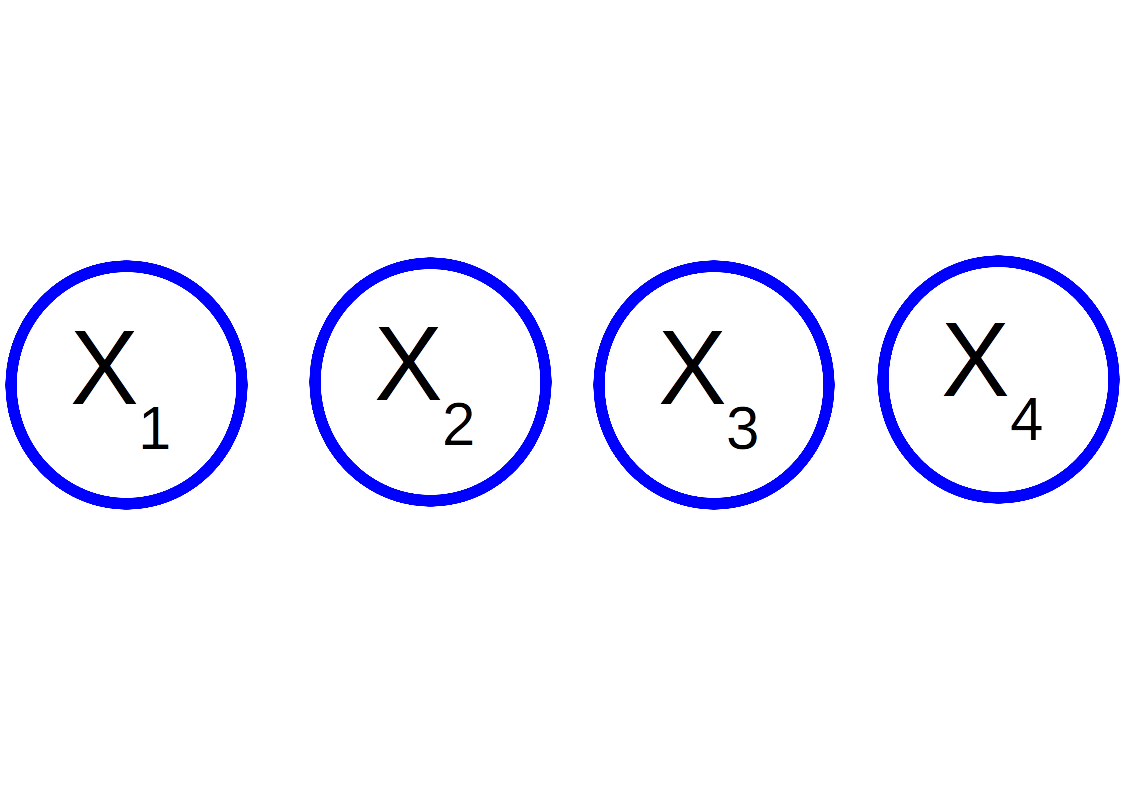
\includegraphics[width=2in,height=2in]{figures/idd.png}
  \end{figure}
\end{frame}

%-------------------------------------------------------
\begin{frame}{Big Picture}{Whey do we need Markov and Hidden Markov Models?}
%-------------------------------------------------------
  \begin{itemize}
    \item What are going to happend if observation are dependent?
    \item How can we calculate the "likelihood" of the sample?
  \end{itemize}
  \begin{figure}[h]
    \centering
    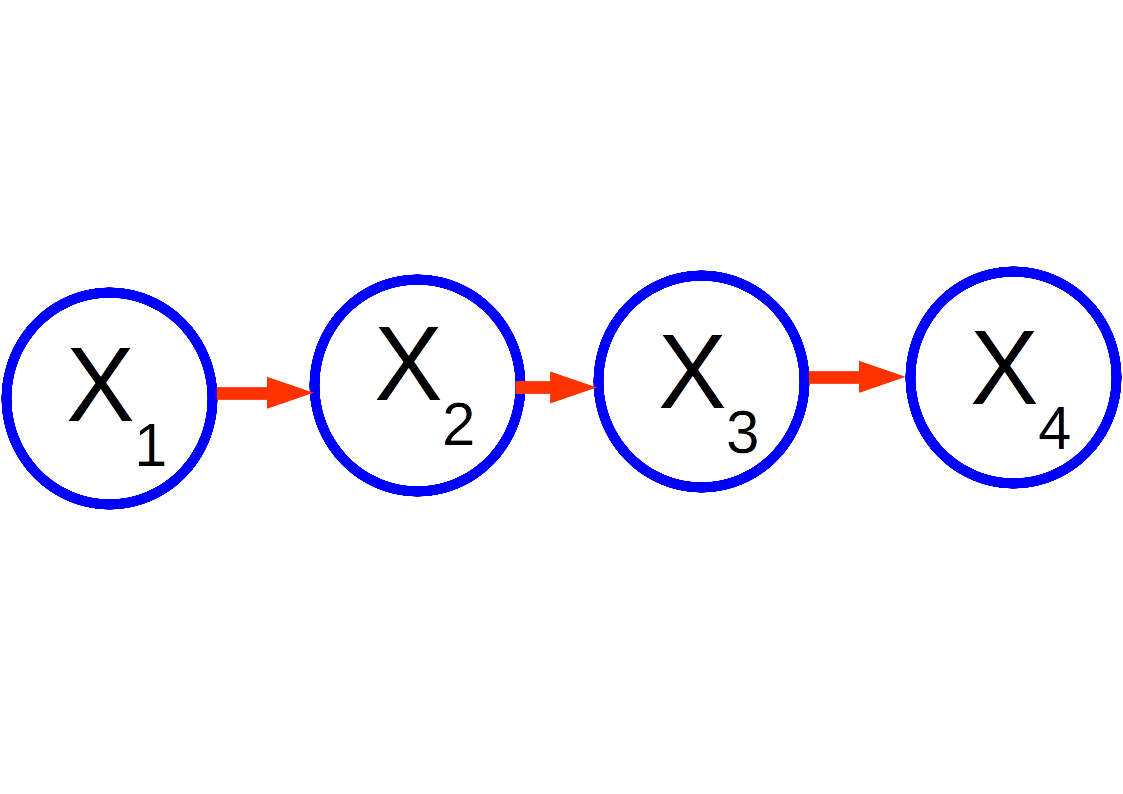
\includegraphics[width=2in,height=2in]{figures/not_idd.png}
  \end{figure}
  \begin{itemize}
    \item What will happend if there is a time correlation between the\
          different samples?\cite{Anders}
  \end{itemize}

\end{frame}

\begin{frame}{Big Picture}{Whey do we need Markov and Hidden Markov Models?}
%-------------------------------------------------------
  \begin{itemize}
    \item How can we predict weather of next day based on weather of today?
  \end{itemize}
  \begin{figure}[h]
    \centering
    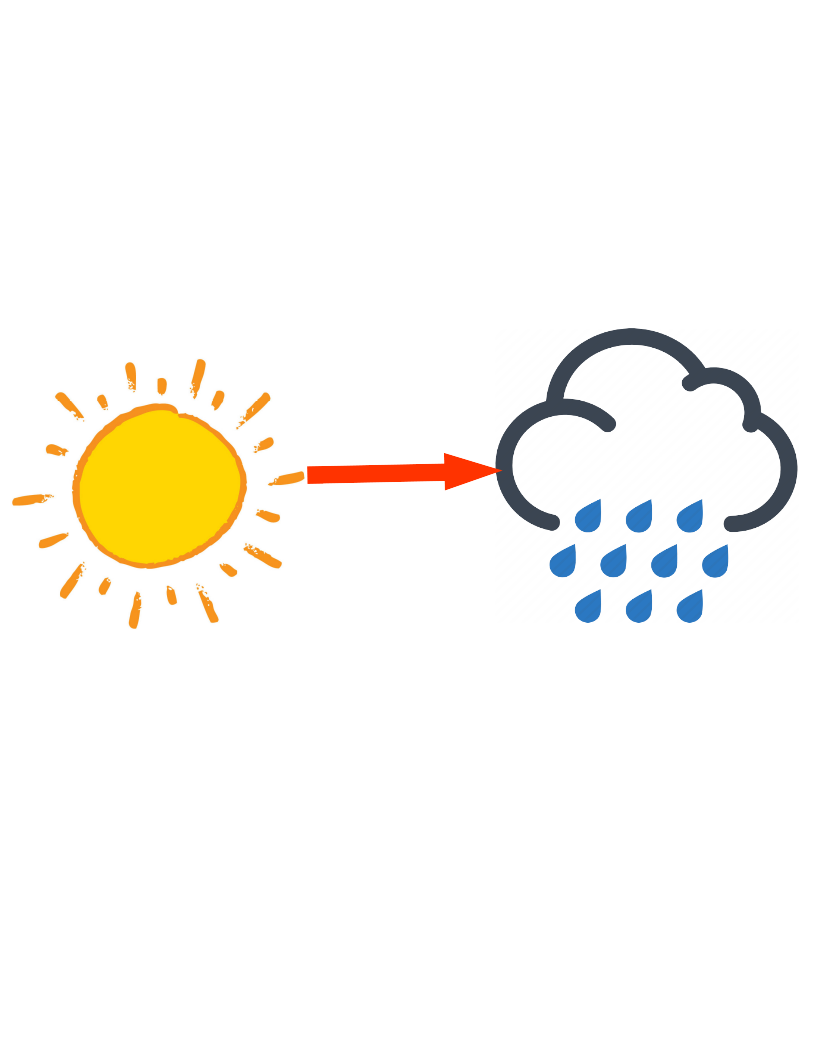
\includegraphics[width=1in,height=1in]{figures/sunny_to_rainny.png}
  \end{figure}
\end{frame}
%-------------------------------------------------------------------------

\begin{frame}{Big Picture}{Whey do we need Markov and Hidden Markov Models?}
%-------------------------------------------------------
  \begin{itemize}
    \item How can we predict weather of next day based on weather of today?
  \end{itemize}
  \begin{figure}[h]
    \centering
    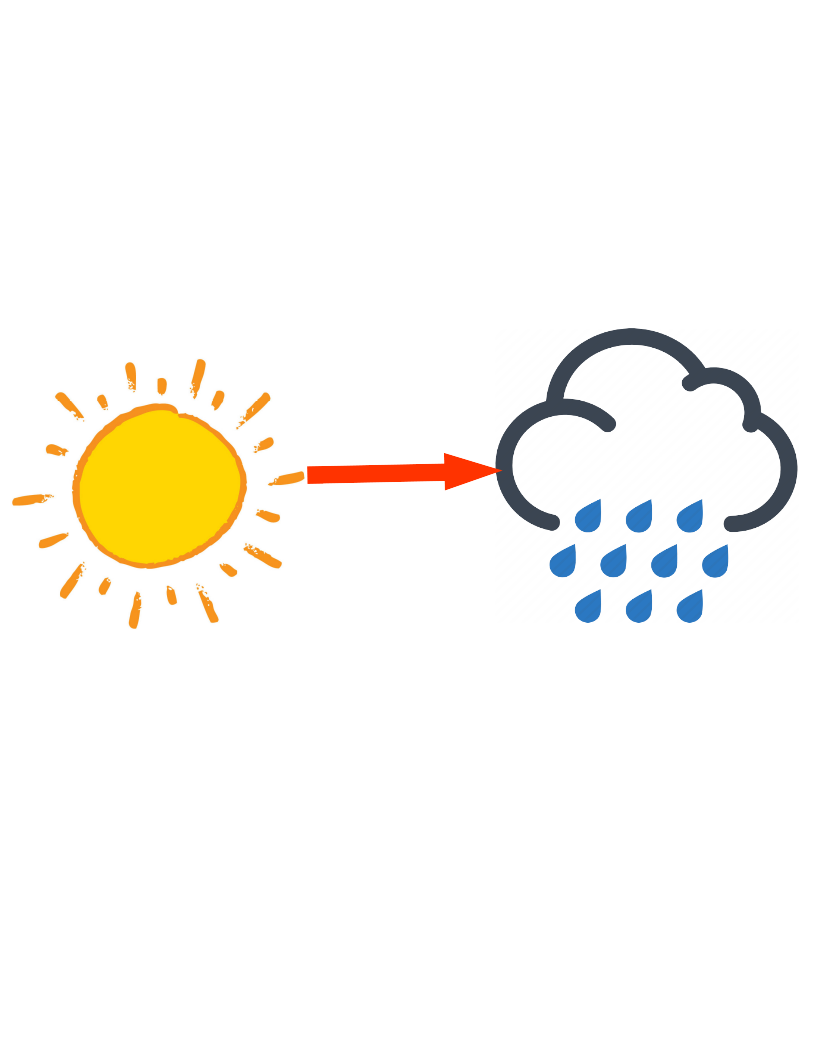
\includegraphics[width=1in,height=1in]{figures/sunny_to_rainny.png}
  \end{figure}
\end{frame}

\begin{frame}{Big Picture}{Whey do we need Markov and Hidden Markov Models?}
%-------------------------------------------------------
  \begin{itemize}
    \item Assume that you have been locked into a room for serveral days, \
          and you have no windows, so can we predict the weather outside \
          based on the clothes of the caretaker?
  \end{itemize}
  \begin{figure}[h]
    \centering
    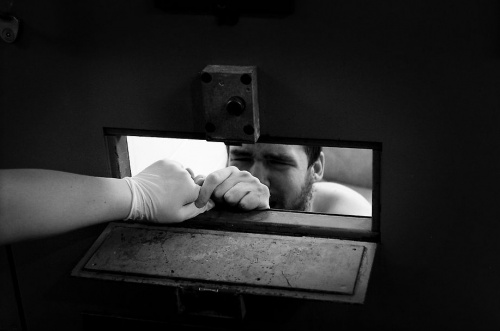
\includegraphics[width=3in,height=2in]{figures/prisoner.jpg}
  \end{figure}
\end{frame}
%-------------------------------------------------------

%-------------------------------------------------------
\section{Markov Model}
%-------------------------------------------------------
\subsection{Ingredients of a Markov Model}
\begin{frame}{Markov Model}{Ingredients}
  \begin{itemize}
    \item States?
    \item States transition probabilities?
    \item Initial state distribution? 
  \end{itemize}
\end{frame}
%-------------------------------------------------------

%-------------------------------------------------------
\begin{frame}{Markov Model}{Weather Example}
%-------------------------------------------------------
  \begin{block}{Weather Example}
     We have 3 states from a weather system $S = \{Sunny, Rainy, Snowy\}$. We \
     observe the weather a few days \
     $\{x_1 = S_{Sun}, x_2 = S_{Rainy}, x_3 = S_{Snowy}\}$
  \end{block}
  \begin{figure}[h]
    \centering
    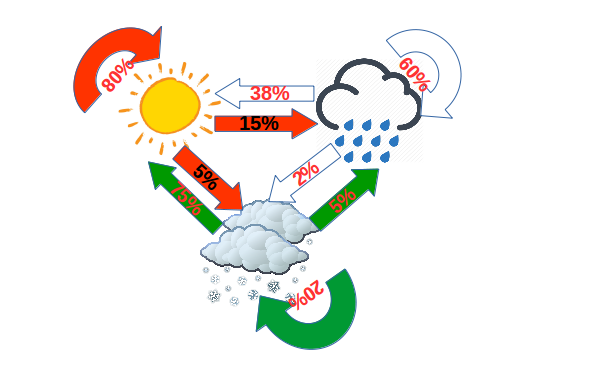
\includegraphics[width=4.5in,height=1.5in]{figures/weather_example.png}
    \caption {Weather: A Markov Model (maybe?)}
  \end{figure}
\end{frame}
%-------------------------------------------------------

%-------------------------------------------------------
\subsection{Markov Assumption}
\begin{frame}{Markov Model}{Markov Assumption}
%-------------------------------------------------------
  \begin{block}{FIRST ORDER MARKOV ASSUMPTION}
        The probability of being in a state at time $t+1$ depends only on the\
        state at time $t$. It means that the state at time $t$ represents\
        "enough" summary of the past to reasonably predict the feature.\cite{Daniel}\\
        Formally:
             $P(x_t|x_{t-1},...,x_1) = P(x_t|x_{t-1})$
  \end{block}
  \begin{block}{STATIONARY PROCESS ASSUMPTION}
       The conditional distribution over next state given current state does \
       not change over time. \cite{Daniel}\\ 
       Formally:
       $P(x_t|x_{t-1}) = P(x_2|x_1);t \in 2..T$
  \end{block}
  \textit{What is the meaning of the \textbf{Stationary Process Assumption}?}\\
  We are going to get back this assumption later!!!!!!!!
\end{frame}
%-------------------------------------------------------

%-------------------------------------------------------
\subsection{Definition}
\begin{frame}{Markov Model}{DEFINITION}
%-------------------------------------------------------
  \begin{block}{Definition(Markov Model)}
     A Markov model is a sequence of random variables \ 
     $x_1,\ x_2,\ x_3,\ ...,\ x_N$, such that the probability\
     distribution of $x_{n+1}$ depends only on the outcome at $x_t$.
  \end{block}
\end{frame}
%-------------------------------------------------------

%-------------------------------------------------------
\subsection{Likelihood Calculation}
\begin{frame}{Markov Model}{Likelihood Calculation}
%-------------------------------------------------------
  \begin{block}{Likelihood Calculation}
  We assump that there are a given sequence of data $D=\{x_1, x_2, ..., x_N\}$ \
  where each of the variables $x_n$ take one of M states $\{S_1, S_2, ..., S_M\}$.
  The likelihood of the sample \textbf{D} can now be calculated as:\\
        \begin{equation}
            p(D|M) = p(x_1 = S_i)\displaystyle \prod_{n=2}^{N}p(x_n = S_j | x_{n-1} = S_i)
        \end{equation}
  \end{block}
\end{frame}
%-------------------------------------------------------

%-------------------------------------------------------
\begin{frame}{Markov Model}{Likelihood Calculation}
  \begin{itemize}
    \item The conditional probabilities $p(x_n = S_j | x_{n-1} = S_i)$ are \
          referred to as \textbf{state transition probabilities} or simple \
          \textbf{transition probabilities}. \cite{Anders}
    \item In most cases we assume that the \textit{transition probabilities} \
          are homogeneous, which means that the probabilities do not change \
          over time(STATIONARY PROCESS ASSUMPTION). \cite{Anders} Formally:
          \begin{equation}
               p(x_n = S_j|x_{n-1} = S_i) = p(x_{n+T} = S_j|x_{n-1+T} = S_i)
          \end{equation}
          Where T is a positive integer larger or equal to one.
  \end{itemize}
\end{frame}
%-------------------------------------------------------

%-------------------------------------------------------
\subsection{Transition Matrix}
\begin{frame}{Markov Model}{Transition Matrix}
%-------------------------------------------------------
  \begin{block}{Transition Matrix}
  The transition probabilites can be written as a transition matrix, which is \
  of dimension $M\ x\ M$. Since each element in the matrix represent a\
  probability of staying or jumping to another state. \cite{Anders}
        \begin{equation}
            A = 
            \begin{bmatrix}
                a_{11} & a_{12} & a_{13}\\
                a_{21} & a_{22} & a_{23}\\
                a_{31} & a_{32} & a_{33}\\
            \end{bmatrix}
        \end{equation}
  \end{block}
  \begin{itemize}
      \item Each entry must be positive, so $a_{i,j} \geqslant 0$ for all i,j.
      \item Each row must sum up to one, since each row represents the\
            probability of jumping from or staying in the state. Formally: \\
            \begin{equation}
               \sum_{j=1}^{M}a_{i,j} = 1\ for\ i\ =\ 1\ ...\ M
            \end{equation} 
  \end{itemize}
\end{frame}
%-------------------------------------------------------

%-------------------------------------------------------
\subsection{Illustration of the Markov Model}
\begin{frame}{Markov Model}{Illustration}
%-------------------------------------------------------
  \begin{figure}[h]
    \centering
    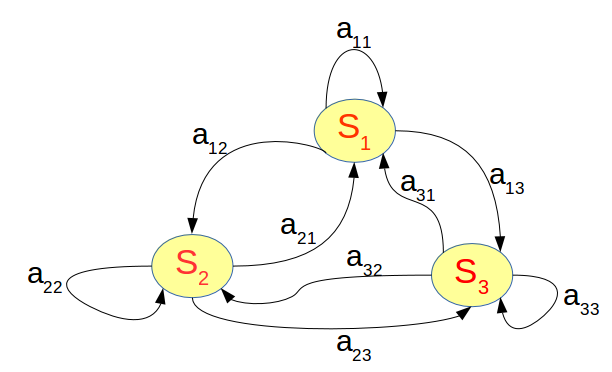
\includegraphics[width=4.5in,height=2.3in]{figures/illustration_markov_model.png}
    \caption {\textbf{Illustration of the Markov Model}}
  \end{figure}
\end{frame}
%-------------------------------------------------------

%-------------------------------------------------------
\begin{frame}{Markov Model}{Graphical Models}
%-------------------------------------------------------
  \begin{itemize}
      \item There is no time information in the illustration.
  \end{itemize}
\end{frame}
%-------------------------------------------------------

%-------------------------------------------------------
\subsection{Illustration of the Markov Model}
\begin{frame}{Markov Model}{Graphical Model}
%-------------------------------------------------------
  \begin{figure}[h]
    \centering
    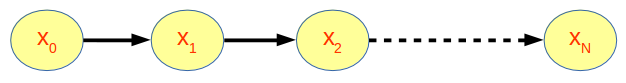
\includegraphics[width=4.6in,height=2.3in]{figures/graphical_models.png}
    \caption {\textbf{Graphical model of Markov Model}}
  \end{figure}
\end{frame}
%-------------------------------------------------------

%-------------------------------------------------------
\subsection{Initial State Probability}
\begin{frame}{Markov Model}{Graphical Model}
%-------------------------------------------------------
  \begin{block}{Transition Matrix}
   To fully characterize the Markov Model, we need to address the 
   \textbf{initial state probability} which is given as \
   $\pi_i(1) = p(x_1 = S_i)$. This probability defines the probability of \
   being in one of the M states at first example. This is also written as a \
   vector:\\
        \begin{equation}
            \pi(1) = [p(x_1 = S_1) p(x_1 = S_2) .. p(x_1 = S_M]^T
        \end{equation}
  \end{block}
\end{frame}
%-------------------------------------------------------

%-------------------------------------------------------
\subsection{Weather Example cont.}
\begin{frame}[allowframebreaks]{Markov Model}{Weather example cont.}
%-------------------------------------------------------
That is enough for theory. Let go back to \textbf{Weather Example}. 
  \begin{figure}[h]
    \centering
    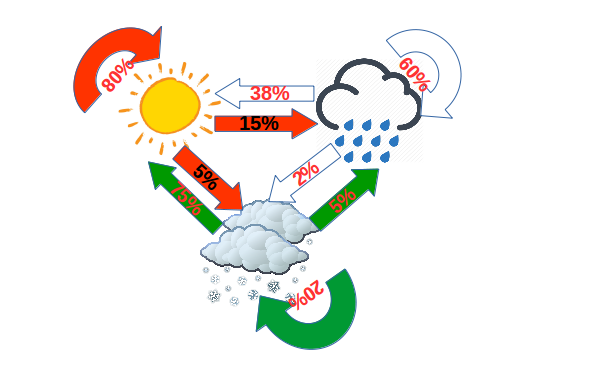
\includegraphics[width=4.6in,height=2.3in]{figures/weather_example.png}
    \caption {\textbf{Weather?A Markov Model?}}
  \end{figure}
  \textbf{Ingredients of a Markov Model}
  \begin{itemize}
      \item States: $\{S_{Sunny},\ S_{rainy},\ S_{snowy}\}$
      \item State transition probabilities:
            \begin{center}
              \begin{tabular}{ |p{2cm}|p{1.2cm}|p{1.2cm}|p{1.2cm}| }
                \hline
                 \multicolumn{4}{|c|}{Weather Markov Model} \\
                \hline
                        & Sunny & Rainy & Snowy \\
                \hline
                     Sunny & 0.8  & 0.15 & 0.05\\
                     Rainy & 0.38 & 0.6  & 0.02\\
                     Snowy & 0.75 & 0.05 & 0.2\\
                \hline
              \end{tabular}
              \end{center}
      \item On assumption, initial state distribution: $\pi = (0.7\ \ 0.25\ \ 0.05)$
  \end{itemize}
  \begin{figure}[h]
    \centering
    
\includegraphics[width=3.5in,height=1.5in]{figures/weather_example_2.png}
    \caption {\textbf{What is the probability of this series?}}
  \end{figure}
   \begin{block}{Solution}
       \fontsize{7}{10}{$P(S_{sunny}).P(S_{rainy}|S_{sunny}).P(S_{rainy}|S_{rainy}).P(S_{rainy}|S_{rainy})$}\
       $.P(S_{snowy}|S_{rainy}).P(S_{snowy}|S_{snowy})$\\
       $=0.7\cdot0.15\cdot0.6\cdot0.6\cdot0.02\cdot0.2=0.0001512$
   \end{block}
\end{frame}
%-------------------------------------------------------

{\1
\begin{frame}[plain,noframenumbering]
  \finalpage{Thanks for your attention}
\end{frame}}

\end{document}
